\documentclass[10pt,a4paper]{article}
\usepackage[utf8]{inputenc}
\usepackage[german]{babel}
\usepackage{mathrsfs}
\usepackage{amsmath}
\usepackage{amsfonts}
\usepackage{amssymb}
\usepackage{amsthm}
\usepackage[left=2cm,right=2cm,top=2cm,bottom=2cm]{geometry}
\usepackage{graphicx}
\usepackage{listings}

\begin{document}

\section{Aufgabe 1}

\subsection{Teil a}

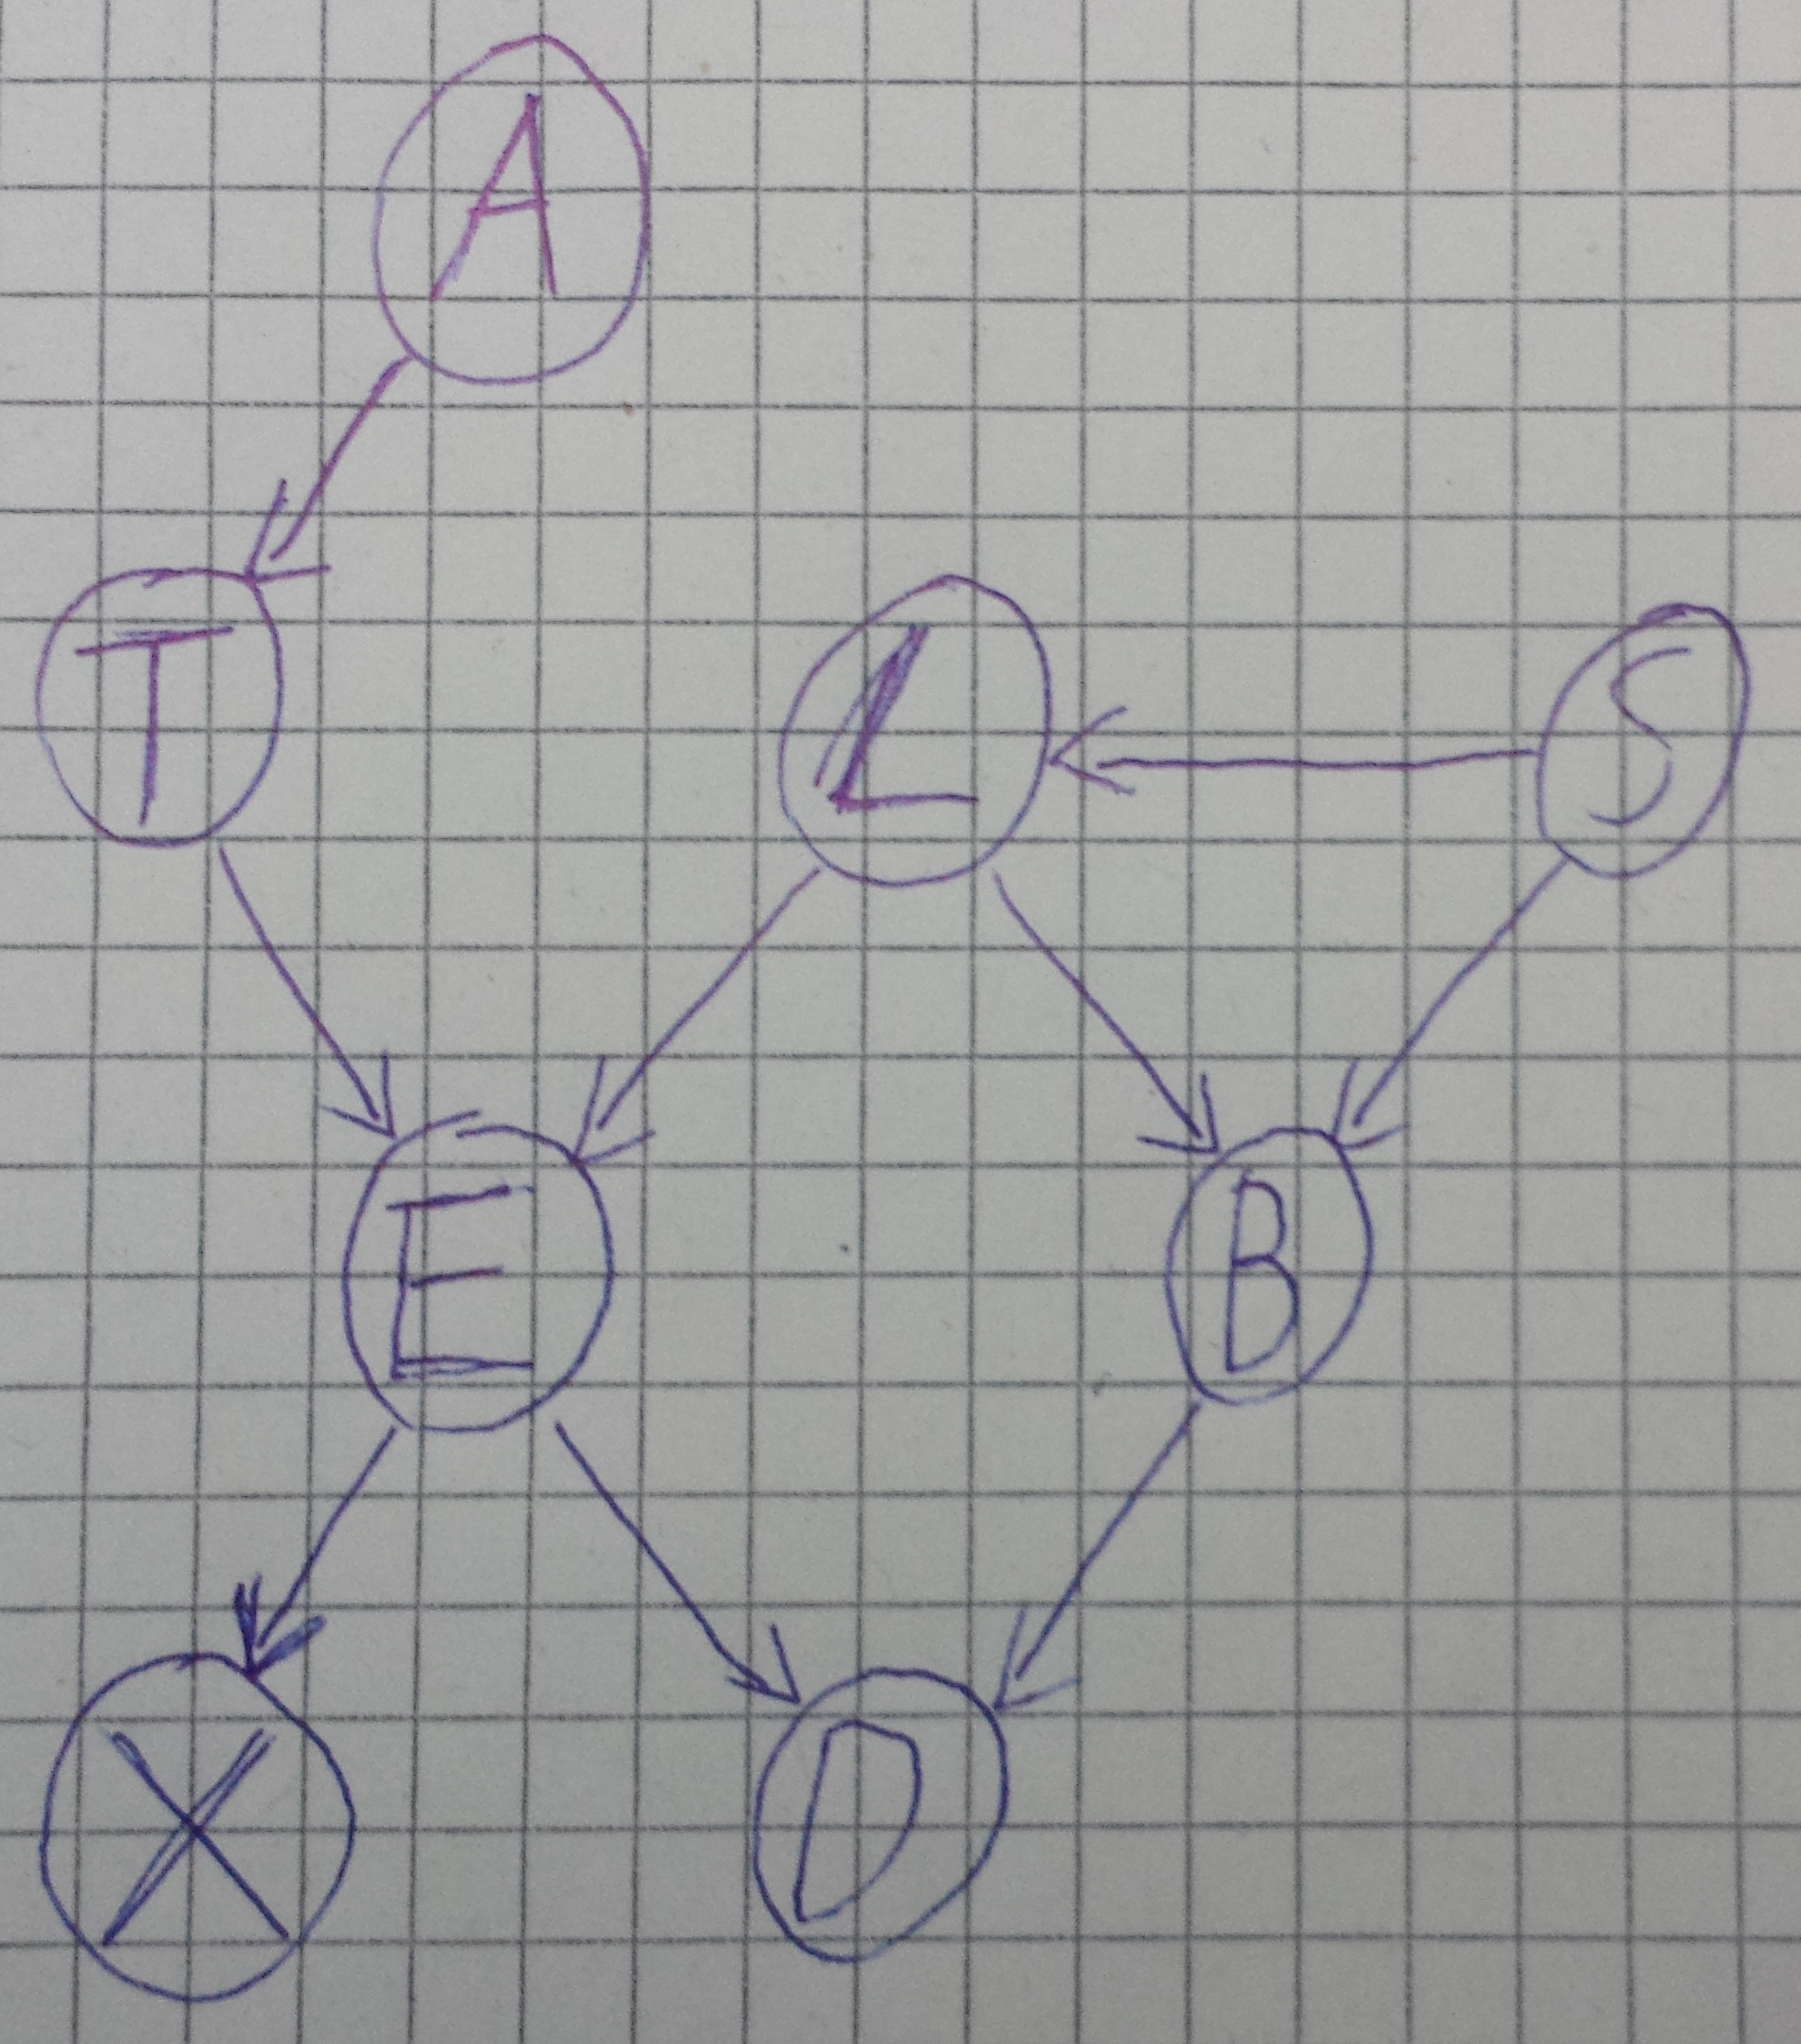
\includegraphics[width=300pt]{2_1_a.png}
\\
Zwischen L und B ist doch kein Pfeil. Habe mich verguckt.

\begin{equation}
  p(X, D, E, T, L, B, A, S) = p(X | E) \cdot p(D | E, B) \cdot p(E | T, L) \cdot p(B | S) \cdot p(T | A) \cdot p(L | S) \cdot p(A) \cdot p(S)
\end{equation}

Program used for the evaluation of the joint distribution written in clojure.
\begin{lstlisting}
(def net
  {[:A []] 0.01
   [:S []] 0.5
   [:T [true]] 0.05
   [:T [false]] 0.01
   [:L [true]] 0.1
   [:L [false]] 0.01
   [:B [true]] 0.6
   [:B [false]] 0.3
   [:X [true]] 0.98
   [:X [false]] 0.05
   [:D [true true]] 0.9
   [:D [true false]] 0.7
   [:D [false true]] 0.8
   [:D [false false]] 0.1
   [:E [true true]] 1
   [:E [true false]] 1
   [:E [false true]] 1
   [:E [false false]] 0})

(defn p
  ([sym yes?]
     (p sym yes? []))
  ([sym yes? params]
     (if yes?
       (net [sym params])
       (- 1 (net [sym params])))))

(defn sum [elements]
  (apply + elements))

(let [S false
      D true]
  (*
   (p :S S)
   (sum (for [X [true false]
              E [true false]]
          (*
           (p :X X [E])
           (sum (for [B [true false]]
                  (*
                   (p :D D [E B])
                   (p :B B [S])
                   (sum (for [T [true false]
                              L [true false]]
                          (*
                           (p :E E [T L])
                           (p :L L [S])
                           (sum (for [A [true false]]
                                  (*
                                   (p :T T [A])
                                   (p :A A)))))))))))))))
\end{lstlisting}

\subsection{Teil b}

\begin{align*}
  p(D) & = p(D | S) \cdot p(S) + p(D | \lnot S) \cdot p(\lnot S)\\
  & = p(D | S) \cdot 0.5 + p(D | \lnot S) \cdot 0.5\\
  & \simeq 0.5528 \cdot 0.5 + 0.31934 \cdot 0.5 = 0.43607
\end{align*}

\subsection{Teil c}

\begin{align*}
  p(D, S) & = \sum_{X, E, T, L, B, A} p(X, D, E, T, L, B, A, S)\\
  & = \sum_{X, E, T, L, B, A} p(X | E) \cdot p(D | E, B) \cdot p(E | T, L) \cdot p(B | S) \cdot p(T | A) \cdot p(L | S) \cdot p(A) \cdot p(S)\\
  & = \sum_{X} \sum_{E} \sum_{T} \sum_{L} \sum_{B} \sum_{A} p(X | E) \cdot p(D | E, B) \cdot p(E | T, L) \cdot p(B | S) \cdot p(T | A) \cdot p(L | S) \cdot p(A) \cdot p(S)\\
  & = p(S) \cdot \sum_{X} \sum_{E} p(X | E) \cdot \sum_{B} p(D | E, B) \cdot p(B | S) \cdot \sum_{T} \sum_{L} p(E | T, L) \cdot p(L | S) \cdot \sum_{A} p(T | A) \cdot p(A)\\
  & \simeq 0.2764
\end{align*}

\begin{align*}
  p(D | S) & = \frac{p(D, S)}{p(S)}\\
  & \simeq \frac{0.2764}{0.5} = 0.5528
\end{align*}

\subsection{Teil d}

\begin{align*}
  p(D, \lnot S) & = p(\lnot S) \cdot \sum_{X} \sum_{E} p(X | E) \cdot \sum_{B} p(D | E, B) \cdot p(B | \lnot S) \cdot \sum_{T} \sum_{L} p(E | T, L) \cdot p(L | \lnot S) \cdot \sum_{A} p(T | A) \cdot p(A)\\
  & \simeq 0.15967
\end{align*}

\begin{align*}
  p(D | \lnot S) & = \frac{p(D, \lnot S)}{p(\lnot S)}\\
  & \simeq \frac{0.15967}{0.5} = 0.31934
\end{align*}

\section{Aufgabe 2}

\begin{equation}
  p(A, C | B) = \frac{p(A, B, C)}{p(B)} \Leftrightarrow p(B) = \frac{p(A, B, C)}{p(A, C | B)}
\end{equation}

\subsection{Teil a}

\begin{equation}
  p(B | A) = \frac{p(A | B) \cdot p(B)}{p(A)} \Leftrightarrow p(A) = \frac{p(A | B) \cdot p(B)}{p(B | A)}
\end{equation}

\begin{align*}
  p(A, B, C) & = p(A) \cdot p(B | A) \cdot p(C | B)\\
  \Leftrightarrow p(A, B, C) & = \frac{p(A | B) \cdot p(B)}{p(B | A)} \cdot p(B | A) \cdot p(C | B)\\
  \Leftrightarrow p(A, B, C) & = p(B) \cdot p(A | B) \cdot p(C | B)\\
  \Leftrightarrow p(A, B, C) & = \frac{p(A, B, C)}{p(A, C | B)} \cdot p(A | B) \cdot p(C | B)\\
  \Leftrightarrow p(A, C | B) & = p(A | B) \cdot p(C | B)
\end{align*}

\subsection{Teil b}

\begin{equation}
  p(B | C) = \frac{p(C | B) \cdot p(B)}{p(C)} \Leftrightarrow p(C) = \frac{p(C | B) \cdot p(B)}{p(B | C)}
\end{equation}

\begin{align*}
  p(A, B, C) & = p(C) \cdot p(B | C) \cdot p(A | B)\\
  \Leftrightarrow p(A, B, C) & = \frac{p(C | B) \cdot p(B)}{p(B | C)} \cdot p(B | C) \cdot p(A | B)\\
  \Leftrightarrow p(A, B, C) & = p(C | B) \cdot p(B) \cdot p(A | B)\\
  \Leftrightarrow p(A, B, C) & = p(C | B) \cdot \frac{p(A, B, C)}{p(A, C | B)} \cdot p(A | B)\\
  \Leftrightarrow p(A, C | B) & = p(A | B) \cdot p(C | B)
\end{align*}

\subsection{Teil c}

\begin{equation}
  p(A, B, C) = p(B) \cdot p(A | B) \cdot p(C | B) = \frac{p(A, B, C)}{p(A, C | B)} \cdot p(A | B) \cdot p(C | B) \Leftrightarrow p(A, C | B) = p(A | B) \cdot p(C | B)
\end{equation}

\subsection{Teil d}

\begin{equation}
  p(A, B, C) = p(A) \cdot p(C) \cdot p(B | A, C) = p(A) \cdot p(C) \cdot \frac{p(A, B, C)}{p(A, C)} \Leftrightarrow p(A, C) = p(A) \cdot p(C)
\end{equation}

\section{Aufgabe 3}

\begin{equation}
  p(A) = p(B) = p(C) = \frac{1}{2}
\end{equation}

I will assume, that $A$, $B$ and $C$ are pairwise indepent, as stated on the
slides. If it was not stated, you could easily see it, by enumerating all cases.

\subsection{Teil a}

\begin{equation}
  p(B | C) = \frac{p(B, C)}{p(C)} = \frac{p(B)p(C)}{p(C)} = p(B)
\end{equation}

\subsection{Teil b}

\begin{equation}
  p(C | A) = \frac{p(C, A)}{p(A)} = \frac{p(C)p(A)}{p(A)} = p(C)
\end{equation}

\subsection{Teil c}

\begin{equation}
  p(A | B) = \frac{p(A, B)}{p(B)} = \frac{p(A)p(B)}{p(B)} = p(A)
\end{equation}

\section{Aufgabe 4}

\begin{equation}
  f(x) = ax + b
\end{equation}
\begin{equation}
  f^{-1}(y) = \frac{y - b}{a}
\end{equation}
\begin{equation}
  \mu_{y} = a\mu + b
\end{equation}
\begin{equation}
  \sigma_{y}^{2} = a^{2}\sigma^{2}
\end{equation}
\begin{equation}
  p_{y}(y) = p_{x}(f^{-1}(y)) = p_{x}\left( \frac{y - b}{a} \right) = N\left( \frac{y - b}{a}; \mu, \sigma^{2} \right) = N(y; a\mu + b, a^{2}\sigma^{2})
\end{equation}

\end{document}